\documentclass[a4paper,11pt]{report}

\usepackage[a4paper,left=2.5cm,right=2.5cm,top=3.5cm,bottom=3.5cm]{geometry}
\usepackage[utf8]{inputenc}
\usepackage[T1]{fontenc}
\usepackage[english]{babel}
\usepackage{graphicx}
\usepackage{amsmath,amssymb,amsthm,amsopn}
\usepackage{mathrsfs}
\usepackage{graphicx}
\usepackage{array}
\usepackage{makecell}
\usepackage{bm}
\usepackage{hyperref}
\usepackage[shortlabels]{enumitem}
\hypersetup{
    colorlinks=true,
    linkcolor=blue,
    citecolor=red,
}
\usepackage{diagbox}

\usepackage{algorithm}
\usepackage{algpseudocode}

\renewcommand{\algorithmicrequire}{\textbf{Input:}}
\renewcommand{\algorithmicensure}{\textbf{Output:}}

%\usepackage[top=1cm,bottom=1cm]{geometry}
%\usepackage{listings}
%\usepackage{xcolor}

\usepackage{tikz}
\usetikzlibrary{arrows}
\usetikzlibrary{math}
\usetikzlibrary{calc}
\usetikzlibrary{decorations.text}

% Tikz style

\tikzset{round/.style={circle, draw=black, very thick, scale = 0.7}}
\tikzset{arrow/.style={->, >=latex}}
\tikzset{possible-arrow/.style={->, >=latex, color=gray!35, thick}}
\tikzset{dashed-arrow/.style={->, >=latex, dashed}}
\tikzset{dotstyle/.style={circle, inner sep = 1.2pt, outer sep = 4pt, fill = gray},
         edgetower/.style={thick},
         edgecomp/.style={thick, lightgray}}
\tikzset{additive-structure/.style={very thick, red!50}}
\tikzset{multiplicative-structure/.style={very thick, blue!50}}
\tikzset{curved text/.style={decorate,
        decoration={text effects along path,
            text={#1}, text align=center,
            text effects/.cd, text along path}}}

% New command
\newcommand{\drawrec}[3]{
  \ifthenelse{\equal{#1}{1}}{
    \fill (#2,#3) -- ++(1,0) -- ++(0, 1) -- ++(-1, 0) -- cycle;
    }
    {
      \tikzmath{\x = #2; \y = #3; \a = #1;
                \b =\a/2; \xx = \x+\b; \yy = \y+\b; }

      \drawrec{\b}{\x}{\y}
      \drawrec{\b}{\xx}{\y}
      \drawrec{\b}{\x}{\yy}
    }
}

%\newtheoremstyle{break}%
%{}{}%
%{\itshape}{}%
%{\bfseries}{}%  % Note that final punctuation is omitted.
%{\newline}{}

%\newtheoremstyle{sc}%
%{}{}%
%{}{}%
%{\scshape}{}%  % Note that final punctuation is omitted.
%{\newline}{}

%\theoremstyle{break}
\theoremstyle{plain}
\newtheorem{thm}{Theorem}[section]
\newtheorem{lm}[thm]{Lemma}
\newtheorem{prop}[thm]{Proposition}
\newtheorem{cor}[thm]{Corollary}

%\theoremstyle{sc}
%\newtheorem{exo}{Exercice}

\theoremstyle{definition}
\newtheorem{defi}[thm]{Definition}
\newtheorem{ex}[thm]{Example}

\theoremstyle{remark}
\newtheorem{rem}[thm]{Remark}

% Math Operators

\DeclareMathOperator{\Card}{Card}
\DeclareMathOperator{\Gal}{Gal}
\DeclareMathOperator{\Id}{Id}
\DeclareMathOperator{\Img}{Im}
\DeclareMathOperator{\Ker}{Ker}
\DeclareMathOperator{\Minpoly}{Minpoly}
\DeclareMathOperator{\Mod}{mod}
\DeclareMathOperator{\Ord}{Ord}
\DeclareMathOperator{\ppcm}{ppcm}
\DeclareMathOperator{\tr}{Tr}
\DeclareMathOperator{\Vect}{Vect}
\DeclareMathOperator{\Span}{Span}
\DeclareMathOperator{\rank}{rank}
\DeclareMathOperator{\ev}{ev}

% Shortcuts

\newcommand{\dE}{\partial(E)}
\newcommand{\dF}{\partial(F)}
\newcommand{\dG}{\partial(G)}
\newcommand{\diff}{\mathop{}\!\mathrm{d}}
\newcommand{\eg}{\emph{e.g. }}
\newcommand{\emb}{\hookrightarrow}
\newcommand{\embed}[2]{\phi_{#1\hookrightarrow#2}}
\newcommand{\ent}[2]{[\![#1,#2]\!]}
\newcommand{\ie}{\emph{i.e. }}
\newcommand{\ps}[2]{\left\langle#1,#2\right\rangle}
\newcommand{\eqdef}{\overset{\text{def}}{=}}
\newcommand{\f}{f}%{\mathfrak{f}}
\newcommand{\bff}{\mathbf{f}}
\newcommand{\E}{\mathcal{E}}
\newcommand{\M}{\mathcal{M}}
\newcommand{\A}{\mathcal{A}}
\newcommand{\B}{\mathcal{B}}
\newcommand{\R}{\mathcal{R}}
\newcommand{\bfa}{\mathbf{a}}
\newcommand{\bfb}{\mathbf{b}}
\newcommand{\D}{\mathcal{D}}
\newcommand{\Pcal}{\mathcal{P}}
\newcommand{\musym}{\mu^{\textrm{sym}}}
\newcommand{\mutri}{\mu^{\textrm{tri}}}
\newcommand{\muhyp}{\mu^{\textrm{hyp}}}
\newcommand{\musymG}[1][G]{\mu^{\textrm{sym},#1}}
\newcommand{\mutriG}[1][G]{\mu^{\textrm{tri},#1}}
\newcommand{\muhypG}[1][G]{\mu^{\textrm{hyp},#1}}
\newcommand{\hmusym}{\hat\mu^{\textrm{sym}}}
\newcommand{\hmutri}{\hat\mu^{\textrm{tri}}}
\newcommand{\hmuhyp}{\hat\mu^{\textrm{hyp}}}
\newcommand{\hmusymG}[1][G]{\hat\mu^{\textrm{sym},#1}}
\newcommand{\hmutriG}[1][G]{\hat\mu^{\textrm{tri},#1}}
\newcommand{\hmuhypG}[1][G]{\hat\mu^{\textrm{hyp},#1}}
\newcommand{\Msym}{M^{\textrm{sym}}}
\newcommand{\Mtri}{M^{\textrm{tri}}}
\newcommand{\Mhyp}{M^{\textrm{hyp}}}
\newcommand{\hMsym}{\hat{M}^{\textrm{sym}}}
\newcommand{\hMtri}{\hat{M}^{\textrm{tri}}}
\newcommand{\hMhyp}{\hat{M}^{\textrm{hyp}}}
\newcommand{\tri}[2]{\mu_{#1}^{\text{tri}}(#2)}
\newcommand{\sym}[2]{\mu_{#1}^{m_3}(#2)}
\newcommand{\K}{\mathbf{k}}


% opening
\title{Efficient arithmetic for cryptography and cryptanalysis}
\author{Édouard Rousseau}



\begin{document}

\maketitle

%\begin{abstract}

%\end{abstract}

\dominitoc
\tableofcontents

%\clearpage

\chapter{Introduction}
This introduction is intended to all readers, not only mathematicians. We
first present some applications of the concept at the center of this thesis, the
\emph{finite field} structure, in order to grasp how useful it is in real life.
Those eager to learn more about the technical details or the mathematics behind
the exposed subjects can do so by reading the articles and books for which we
give references. Of course, this thirst for mathematics can also be fulfilled
(up to a point) by reading the next chapters of this thesis.

\minitoc
% TODO
% ====
%
% Find an illustration (something linked with crypto preferably)
\clearpage

\section{Applications of finite fields}

During my PhD, I would always explain to non-mathematicians that I was doing a
PhD in \emph{cryptography}. This is in fact a lie, because even if
the words ``cryptography'' and ``cryptanalysis'' were initially among those composing
the title of this project, that was first called \emph{Efficient arithmetic for
cryptography and cryptanalysis}, the thesis is definitely more oriented
towards the two first words: \emph{efficient arithmetic}. Still, cryptography
is one of the motivations and sometimes inspiration for this work. The problems
we focus on either have their roots or have applications in cryptography, thus
we begin by explaining what it is.

\subsection{Cryptography}
\label{sec:crypto}

As we are social animals, we often need to communicate with each other.
Sometimes, we want our communications to be secret: the reasons behind this
wish are multiple: military information, business, secret love stories, banking
information, personal medical information, and so on... Cryptography is the
practice and study of the techniques used to secure communications, in the
presence of third parties called \emph{adversaries}. Historically, cryptography
focused on \emph{encryption} of messages (message confidentiality), \ie making
the message unreadable for someone intercepting or eavesdropping it. For the
rightful recipient of the message to be able to read the message, he or she had
to be able to \emph{decrypt} (we also say \emph{decipher}) the message. It was
only possible when both the sender and the receiver of the message shared a
secret beforehand, the secret was then used to both cipher and decipher the
message. In a cryptographic protocol, the common secret is called a
\emph{key}, because the encryption is viewed as some padlock. This encryption
method is called \emph{symmetric cryptography} because both participants share
the same key. The situation is summed up in Figure~\ref{fig:crypto-sym}.
\begin{figure}[h]
  \centering
  \begin{tikzpicture}
    \node (msg) at (0,0) {Message};
    \node (msg-enc) at (6,0) {Encrypted message};
    \node (msg-rec) at (12,0) {Message};
    \node (secret) at (6, 2) {Secret};
    \node (enc) at (2.15,1.8) {Encryption};
    \node (dec) at (9.75,1.8) {Decryption};

    \draw[->] (msg) -- (msg-enc);
    \draw[->] (msg-enc) -- (msg-rec);
    \draw[->] (secret) to[bend right] (2.2,0);
    \draw[->] (secret) to[bend left] (9.8,0);
    \node (a) at (2.2,1) {\includegraphics[scale=0.3]{img/key-128.png}};  
    \node (b) at (9.8,1) {\includegraphics[scale=0.3]{img/key-128.png}};  
    \node (c) at (6,-1) {\includegraphics[scale=0.05]{img/lock-128.png}};  
  \end{tikzpicture}
  \caption{The general strategy of a symmetric cryptography protocol.}
  \label{fig:crypto-sym}
\end{figure}
One famous example of an old cryptography protocol is the Caesar cipher, in
which each letter of the message is replaced by another letter. All the letters
are shifted by a constant number $n$ of positions down the alphabet. For
example, with $n=3$, the letter \texttt{D} becomes \texttt{A}, the letter
\texttt{E} becomes \texttt{B}, the letter \texttt{F} becomes \texttt{C}, and so
on. This encryption protocol is named after Julius Caesar,
who was using it to communicate with his generals with the shift $n=3$. In
Figure~\ref{fig:caesar}, we draw the correspondence between the letters using
the shift $n=3$. The outer ring represent the letters in the \emph{plaintext}
(the original text, without encryption) while the inner ring represent the
letters in the \emph{ciphertext} (the text after the encryption).
\begin{figure}[h]
  \centering
  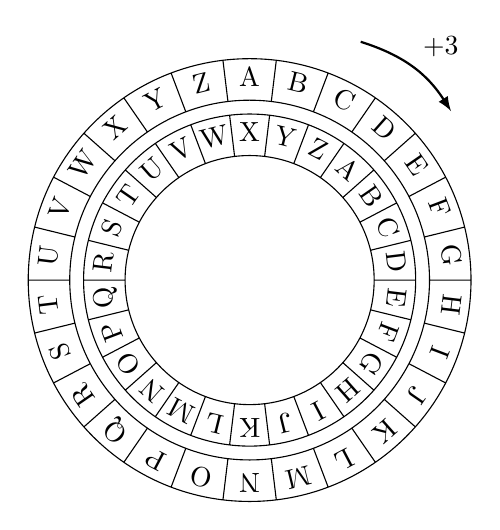
\begin{tikzpicture}[x=1em,y=1em]
%   set up
    \pgfmathsetmacro\angdiv{360/26}
    \pgfmathtruncatemacro\caeser{3} % Input Caeser shift here! (positive for clockwise)
    \coordinate (n-0) at (90+\angdiv/2:7) {};
    \coordinate (m-0) at (90-\caeser*\angdiv+\angdiv/2:5) {};
%   draw Caeser diagram
    \draw circle [radius=8] circle [radius=6.5] circle [radius=6]  circle [radius=4.5]
        \foreach \i in {0,...,25}{%
            ($({90-(\i-1/2)*\angdiv}:8)$) -- ($(({90-(\i-1/2)*\angdiv}:6.5)$)
            ($({90-(\i-1/2)*\angdiv}:4.5)$) -- ($(({90-(\i-1/2)*\angdiv}:6)$)
        };
    \foreach [count=\a from 0] \text in {A,B,...,Z}{
        \pgfmathtruncatemacro\b{\a+1}%
        \path [curved text=\text] (n-\a) arc [start angle=90-(\a-1/2)*\angdiv, delta angle=-\angdiv, radius=7] node (n-\b) {};
        \path [curved text=\text] (m-\a) arc [start angle=90-(\a+\caeser-1/2)*\angdiv, delta angle=-\angdiv, radius=5] node (m-\b) {}; % Inner circle
    }
%   draw arrow
    \draw [-latex, thick] (65:9.5) to[bend left=20,edge label=$+3$] (40:9.5);
    \end{tikzpicture}
  \caption{Representation of the Caesar cipher with a shift $n=3$.}
  \label{fig:caesar}
\end{figure}
In this example, the secret key of the protocol is the shift parameter $n$: if
you know $n$, you know both how to encrypt a message and how to decrypt one.
Caesar cipher is simple enough to be executed by a machine, but it is not used
nowadays. Indeed, the number of keys one can choose when using Caesar cipher is
rather small, so an adversary (a spy, an enemy...) can easily guess what it is
after spending enough time trying all the possibilities. One could even ask a
computer to search for all the possible keys, thus recovering it even faster.
That is why, in modern cryptography, the number of possible keys must be way
bigger than this. For example, the standard protocol for symmetric encryption,
called AES (for Advanced Encryption Standard), was designed in 1999~\cite{DR99,
DR02} and can be used with $2^{128}, 2^{192}$ or $2^{256}$ different possible
keys, depending on the version used. The smallest of these number can also be
written as
\[
  2^{128} = 340282366920938463463374607431768211456,
\]
when a billion looks like
\[
  10^{9} = 1000000000,
\]
so they are really big numbers.

The number of possible keys is not the only thing that changed since Julius
Caesar. First, communication is now essentially digital, thus cryptography is
now a part of computer science. This is very important because it means that the
work in this thesis is also oriented towards computer science: we want to obtain
mathematical results that are effective, \ie usable by a computer.
Second, the scope of cryptography is now larger.
In modern cryptography, symmetric encryption is only one field of
cryptography, and there are many more aspects, such as asymmetric
encryption (also called \emph{public-key} encryption), data integrity,
anthentification, digital signatures (the list is not exhaustive). We will not
explain all these terms, but the interested reader can look at the introductions
on each of these subjects in~\cite{MVOV18}, for example. An important change in
cryptography occured in 1976 with the seminal article \emph{New Directions in
Cryptography}~\cite{DH76} by Diffie and Hellman, with the invention of so called
public key cryptography. We briefly present public key encryption, in order to
compare it to symmetric encryption.

One of the main drawback about symmetric encryption is that the two
protagonists must have a secret in common in order to be able to securely
communicate. They can meet in person and agree on a secret, but this is not
always possible, for example if they live very far away of each other. They
could also find another way of communication, but then they cannot encrypt their
communication, because they do not share a secret yet and they want to
communicate precisely in order to share one. Thus, the problem of sharing a
secret seems to be unsolvable. In fact, public key encryption is an answer to
this problem, because it allows to encrypt messages without the need for a
common secret. The elegant idea of Diffie and Hellman is to break the symmetry
between the participants (we will call them Alice and Bob, since it is
traditional to do so in cryptography). Instead of agreeing on a common key, only
one participant (for example Alice) creates a \emph{pair} of keys: one of them
is public and can be transmitted to anyone, while the other is private and must
be known by Alice only. With the public key, one can encrypt a message, while
the private key is necessary in order to decrypt an encrypted message. Using
such a system, everyone is able to send encrypted messages to Alice, because the
key used to do so is public, but only Alice can decrypt them. Thus, the
communications are secure.
\begin{figure}[h]
  \centering
  \begin{tikzpicture}
    \node (msg) at (0,0) {Message};
    \node (msg-enc) at (6,0) {Encrypted message};
    \node (msg-dec) at (12,0) {Decrypted message};
    \node (bob) at (0,2) {Bob};
    \node (alice) at (12, 2) {Alice};
    \node (key-pub) at (5, 2) {\includegraphics[scale=0.3]{img/key-128.png}};
    \node (key-pub-txt) at (5, 3) {Public key};
    \node (key-pri) at (7, 2) {\includegraphics[scale=0.065]{img/key-512.png}};
    \node (key-pri-txt) at (7, 3) {Private key};
    \node (lock) at (6,-1) {\includegraphics[scale=0.05]{img/lock-128.png}};  
    \draw[->] (msg) -- (msg-enc);
    \draw[->] (msg-enc) -- (msg-dec);
    \draw[->] (bob) to[bend left, edge label=Encrypts] (2.5,0);
    \node (key-pub2) at (2.2, .8) {\includegraphics[scale=0.3]{img/key-128.png}};
    \draw[->] (alice) to[bend right, edge label = Decrypts] (9,0);
    \node (key-pri2) at (9.4, .8) {\includegraphics[scale=0.065]{img/key-512.png}};
    \draw[->] (alice) to (8,2);
    \node (c) at (9.5, 2.3) {Creates};
  \end{tikzpicture}
  \caption{General concept of public-key encryption.}
  \label{fig:crypto-asym}
\end{figure}
We draw a diagram of the general idea in Figure~\ref{fig:crypto-asym}. With such
a system, only Bob can send messages to Alice. If Alice wants to send a message
to Bob using public-key cryptography, then Bob has to create his own pair of
keys. He then gives his public key to Alice, who can then encrypt her message
using this key and send it to Bob. Bob decrypts the message using his private
key. Public-key cryptography is somewhat heavier than symmetric
cryptography, hence another solution for Bob is to encrypt a secret and send it
to Alice, in order to be able to use symmetric encryption with that secret. This
is what is done in practice: only a \emph{key exchange} is performed using
public-key cryptography, the rest being handled by symmetric cryptography.
Still, public-key cryptography is foundamental, since it allows us to use
symmetric cryptography.

The first key exchange protocol was invented by Diffie and Hellman in
1976~\cite{DH76}, and an example of public-key encryption is given by the RSA
(named after Rivest, Shamir, and Adleman) protocol~\cite{RSA78} that was
described in 1977. These two protocols are both based on mathematical algebraic
structures. Indeed, mathematics are a handy way of studying and explaining
cryptography, for example Caesar cipher with $n=3$ can be explained by
representing all letters by the numbers between $0$ and $25$
\[
  \texttt{A}\to 0, \texttt{B} \to 1, \dots,\texttt{Y}\to24, \texttt{Z}\to25
\]
and by defining the encryption as the substraction by $3$. With this
representation, we have to agree that the number $-1$ is equivalent to the
number $25$, \ie before \texttt{A} comes \texttt{Z}, that $-2$ is equivalent to
$24$, \ie two times before \texttt{A} comes \texttt{Y}, and so on. In fact a
subpart of mathematics called \emph{number theory} is dedicated to the study of
this kind of numbers, together with some rules like the one that we just stated:
$-1=25$. These sets of numbers are called \emph{cyclic groups}, because they can
be represented on a circle, the one we spoke about is denoted by
\[
  \mathbb{Z}/26\mathbb{Z}
\]
and is represented in Figure~\ref{fig:cyclic-group}.
\begin{figure}[h]
  \centering
  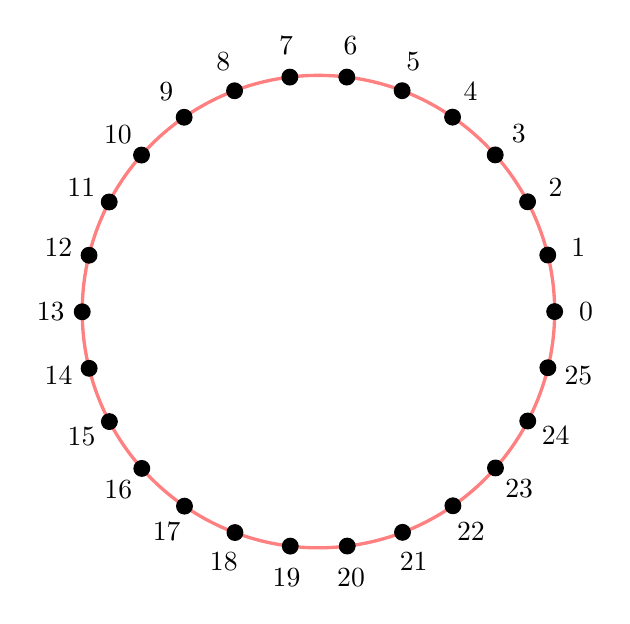
\begin{tikzpicture}
    \foreach \x in {0, 1,...,25} \coordinate (\x) at (13.85*\x:3);
    \draw[additive-structure] (0,0) circle (3);
    \foreach \x in {0, 1,...,25} \draw[fill] (13.85*\x:3) circle (.1);
    \foreach \x in {0, 1,...,25} \node (p) at (13.85*\x:3.4) {$\x$};
  \end{tikzpicture}
  \caption{The cyclic group $\mathbb{Z}/26\mathbb{Z}$ represented on a circle.}
  \label{fig:cyclic-group}
\end{figure}
Many other interesting structures exist, see for example~\cite{Lang04, Perrin96}
for a course in algebra. With the growth of public-key cryptography, number
theory became its corner stone, and more advanced mathematical concepts were
used, like finite fields, elliptic curves or isogenies. Without entering into
the details of what these objects are, what is important is that the security of
cryptographic protocols relies on hard mathematical problems involving these
concepts. Thus, a better understanding of them means a better understanding of
the security of our cryptographic protocols. The part of cryptography that is
dedicated to the study of the security of cryptographic protocols (\ie how to
``break'' them) is called \emph{cryptanalysis}.

At the same time, since the protocols are based on the manipulation of these
objects, a better understanding of them also means better (in particular,
faster) cryptographic protocols. Since cryptography is everywhere in modern
communications (on the Internet, when you use your credit card, on messaging
applications on your smartphone, ...), efficient protocols are crucial. It is
thus necessary to be able to efficiently manipulate the mathematical concepts
behind our protocols both for cryptography (making efficient protocols) and
cryptanalysis (being able to analyze their security). By ``manipulate'', we mean
being able to do additions, multiplications, and sometimes more complicated
operations with these objects: the science studying how to do so is called
\emph{arithmetic}. In conclusion, it is necessary to have efficient arithmetic
for cryptography and cryptanalysis.

\subsection{Coding theory}
\label{sec:coding}

Another very elegant (and useful) application of finite fields is
\emph{coding theory}. Like cryptography, it is linked with communication,
although it adresses a different issue entirely. We now assume that Alice and
Bob want to communicate, and that the information they send go through a
channel. In practice, this channel could be optical fiber, electrical wires, radio
waves, and many more things. Assume that Alice wants to send the message ``Hi!
How are you?'' to Bob. In fact these letters would probably first be translated
into some stream of bits \texttt{0} and \texttt{1}, thus we will imagine that
Alice sends the message
\[
  m = \texttt{0010110001010111}
\]
through the cannel. Very often, in real conditions, the communication channel is
not perfect and is subject to \emph{channel noise}, \ie because of the quality of
the channel, or because of the environment, some errors can appear and change
the message sent by Alice into something else, as shown in
Figure~\ref{fig:communication-channel}.
\begin{figure}[h]
  \centering
  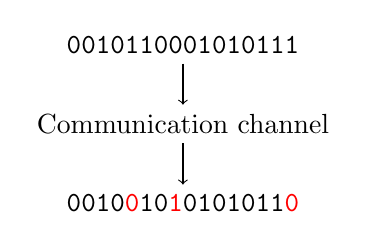
\begin{tikzpicture}
    \node (msg) at (0,2) {\texttt{0010110001010111}};
    \node (msg-dec) at (0,0)
    {\texttt{0010\textcolor{red}{0}10\textcolor{red}{1}0101011\textcolor{red}{0}}};
    \node (channel) at (0, 1) {Communication channel};
    \draw[->] (msg) -- (channel);
    \draw[->] (channel) -- (msg-dec);
  \end{tikzpicture}
  \caption{An imperfect communication channel.}
  \label{fig:communication-channel}
\end{figure}
Without any tool or context, it can be hard (or impossible) for Bob to guess
what was the initial message coming from Alice. Coding theory studies how to
make sure that Bob can recover the original message, even with some errors. The
goal is to build so-called \emph{codes} that can correct errors,
thus they are called \emph{error correcting codes} or \emph{error correction
codes}. The intuition is that in order to make sure that some
information, that is elementary reprensented by a \texttt{0} or a
\texttt{1}, arrives without error to Bob, Alice can just repeat it multiple
times. For example, if Alice repeats every bit three times, making words of
three symbols:
\[
  \texttt{0}\to\texttt{000}\quad\quad\texttt{1}\to\texttt{111},
\]
then an error can be corrected, because if Bob receives, for example, the
word \texttt{001}, he knows that is it most likely coming from
the word \texttt{000}, and he can interpret it as coming from the bit \texttt{0} in
Alice's initial message. More generally, if Bob receives the word
\texttt{abc}, he
interprets it as coming from the symbol \texttt{0} if there is a majority of
\texttt{0} in the word \texttt{abc}. Conversely, if there is a majority of
\texttt{1} in the word \texttt{abc}, he interprets the word as the symbol
\texttt{1}. Of course, if there are too much errors on a single word, it is
still possible to misinterpret it. For example, if the word
\texttt{000} becomes \texttt{110} after going through the communication channel,
then Bob will decode it as $\texttt{111}\to\texttt{1}$. This strategy is known
as the binary repetition code of
length $3$ and is an example of an error correction code. The whole procedure is
described in Figure~\ref{fig:rep3}.
\begin{figure}[h]
  \centering
  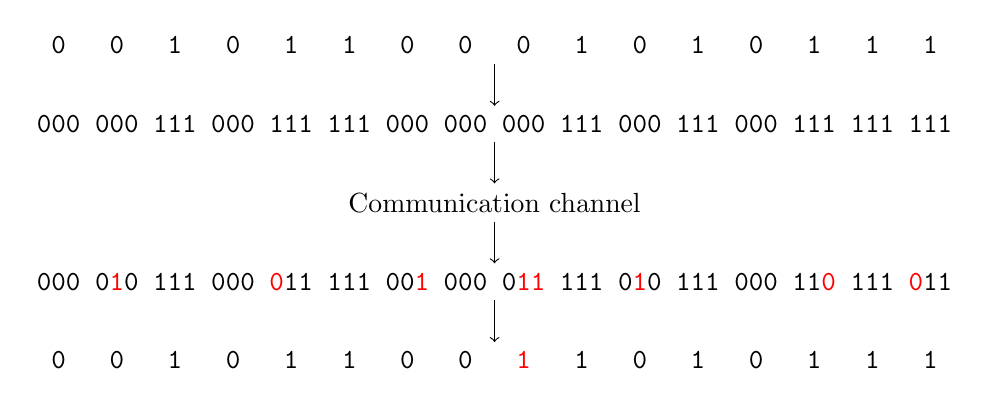
\begin{tikzpicture}
    \node (msg-init) at (0,3)
    {\texttt{\phantom{ }0\phantom{ } \phantom{ }0\phantom{ } \phantom{
    }1\phantom{ }  \phantom{ }0\phantom{ }  \phantom{ }1\phantom{ }  \phantom{
    }1\phantom{ }  \phantom{ }0\phantom{ }  \phantom{ }0\phantom{ }  \phantom{
    }0\phantom{ }  \phantom{ }1\phantom{ }  \phantom{ }0\phantom{ }  \phantom{
    }1\phantom{ }  \phantom{ }0\phantom{ }  \phantom{ }1\phantom{ }  \phantom{
    }1\phantom{ }  \phantom{ }1\phantom{ }}};
    \node (msg) at (0,2)
    {\texttt{000 000 111 000 111 111 000 000 000 111 000 111 000 111 111 111}};
    \node (msg-dec) at (0,0)
  {\texttt{000 0\textcolor{red}{1}0 111 000 \textcolor{red}{0}11 111
  00\textcolor{red}{1} 000 0\textcolor{red}{11} 111 0\textcolor{red}{1}0 111 000 11\textcolor{red}{0} 111 \textcolor{red}{0}11}};
    \node (channel) at (0, 1) {Communication channel};
    \node (msg-end) at (0,-1)
    {\texttt{\phantom{ }0\phantom{ } \phantom{ }0\phantom{ } \phantom{
    }1\phantom{ }  \phantom{ }0\phantom{ }  \phantom{ }1\phantom{ }  \phantom{
    }1\phantom{ }  \phantom{ }0\phantom{ }  \phantom{ }0\phantom{ }  \phantom{
    }\textcolor{red}{1}\phantom{ }  \phantom{ }1\phantom{ }  \phantom{ }0\phantom{ }  \phantom{
    }1\phantom{ }  \phantom{ }0\phantom{ }  \phantom{ }1\phantom{ }  \phantom{
    }1\phantom{ }  \phantom{ }1\phantom{ }}};
    \draw[->] (msg-init) -- (msg);
    \draw[->] (msg) -- (channel);
    \draw[->] (channel) -- (msg-dec);
    \draw[->] (msg-dec) -- (msg-end);
  \end{tikzpicture}
  \caption{The binary repetition code of length $3$.}
  \label{fig:rep3}
\end{figure}
In order to correct more errors, we could use repetition codes with bigger
lengths. Though, when we use a repetition code of length $n$, we have to send
$n$ times more information in the communication channel, which comes at a cost
in real life situations. We thus have to balance the cost coming from the length
of the code with the number of errors we want to be able to correct. In fact,
depending on the quality of the communication channel, all codes are not
suitable. Claude Shannon proved in
1948~\cite{Shannon48} that we can define a quantity called the \emph{capacity}
of the channel that essentially measures how much information we can send
through a communication channel. It also measures how much repetition we
must add in our code in order to send something through the communication
channel in a reliable way. Coding theory is still an active research field, thus
there are plenty of open problems and the question ``What is the best code we
can use?'' has no definitive answer. The codes used in practice
are a bit more subtle that the repetition code, even if they follow the same
logic. Finite fields are used to represent and manipulate codewords of error
correction codes. For example, the Reed-Solomon codes~\cite{RS60}, that are used
in consumer technologies like CDs, DVDs, Blu-ray discs, QR codes, but also in
space NASA missions, use sequences of values taken in a finite field as
codewords. In conclusion, exactly like in cryptography, finite fields are
ubiquitous in coding theory, and efficient arithmetic in finite fields ensures
at the same time fast coding and fast decoding.

\section{Finite fields arithmetic}

As stated in Sections~\ref{sec:crypto} and~\ref{sec:coding}, cryptographic
protocols and codes rely on
mathematical structures in order to work. The one we will study throughout this
document is called \emph{finite field}. A \emph{field} is a mathematical
structure (we also say \emph{algebraic structure}) composed of elements that we
can \emph{add}, \emph{substract}, \emph{multiply}, and \emph{divide} (except by
zero). It is a well-known algebraic structure: for example the set of real
numbers, denoted by $\mathbb{R}$, is a field. Indeed, the elements in
$\mathbb{R}$, for example $0, 1, -3, 5631$ but also more complicated numbers
such as $\pi, \sqrt 2, \frac{7}{13}$ can be added, substracted, multiplied or
divided. Numbers in $\mathbb{R}$ can have an infinite number of decimals, for
example the $60$ first decimals of the constant $\pi$ are
\[
  \pi = 3.14159265358979323846264338327950288419716939937510582097494\dots.
\]
A computer only has a finite memory, \ie the quantity of information it can
store is finite. As a consequence, it is impossible to store all the decimals of
$\pi$, and, more generally, the decimals of a lot of numbers in $\mathbb{R}$. It
is still possible to work with numbers in $\mathbb{R}$ on a computer, but it is
somewhat harder than to work with elements in a \emph{finite} algebraic
structure, \ie a set composed of $n$ elements, with
\[
  n < \infty.
\]
One example of such a structure was given in Section~\ref{sec:crypto}: the
cyclic groupe $\mathbb{Z}/26\mathbb{Z}$ that is composed of the ``numbers'' $0,
1, \dots, 25$. They are not the same numbers as those we know though, since with
the elements of $\mathbb{Z}/26\mathbb{Z}$ we have, for example
\[
  3 - 4 = -1 = 25,
\]
and this is not true for the actual numbers in $\mathbb{R}$, but we still write
them the same way for convenience. We already defined an
addition and substraction on $\mathbb{Z}/26\mathbb{Z}$, and we could also define
a multiplication and a division in a very natural way. Finite fields are a
generalization of spaces like
$\mathbb{Z}/26\mathbb{Z}$. The set $\mathbb{Z}/26\mathbb{Z}$ is not a field for
technical reasons, but to think of finite fields as sets like this is a good
enough approximation for this introduction.

Because the elements of a finite field are, by definition, finite, they are
somewhat easier to manipulate on a computer. Moreover, the field structure
allows us to manipulate the elements like usual numbers (\ie with additions,
multiplications, ...), which makes them useful. This is why today, finite fields
are everywhere in cryptography, but also in other domains at the crossroad of
mathematics and computer science, like coding theory.

Sometimes, simple mathematical problems are well understood on a theoretical
point of view, but there are still open questions concerning practical aspects.
For example, the multiplication of two integers $a$ and $b$ in $\mathbb{N}$ is a
simple problem, that can be done by hand by children. Still, the question of how
to compute it on a computer (in an optimal way) is open, and there are still
research articles~\cite{HVDH19} on that problem.
Finite field arithmetic (\ie how to perform operations such as additions and
multiplications) is very well understood, because the finite field structure is
rather simple. But again, the best way of multiplying two elements in a finite
field is still unknown. This is the subject of this thesis: the study of the
finite field arithmetic.

\section{Organization of the document}
\subsection{Efficient arithmetic in a single finite field}

This work is composed of two parts, that are essentially independent. In
Part~\ref{part:single}, we study the arithmetic of one fixed finite field
extension
\[
  \mathbb{F}_{p^k}.
\]
\paragraph{Preliminaries.} We begin in Chapter~\ref{chap:preliminary} by
recalling foundamental
facts about the mathematical objects that we use in the rest of the document. We
present some properties about \emph{finite fields}, that are at the center of
this thesis. In particular, we recall the structure of finite fields, and how to
construct them as quotients of polynomial rings
\[
  \mathbb{F}_p[x]/(P(x)).
\]
We also give some properties of finite field extensions concerning their vector
space structure and their group of automorphisms.

In Section~\ref{sec:algebraic-function-fields}, we present \emph{algebraic
function fields}, an algebraic structure that we use in some proofs in
Chapters~\ref{chap:bilinear} and~\ref{chap:hypersymmetric}. We briefly recall
what \emph{places} are, and that they are essentially equivalent to a discrete
valuation or a valuation ring. We describe how to evaluate an element
$z$ of the algebraic function field to a place $P$, and give the definition of
zero and pole, justifying the name of ``function'' field. We finally give the
definition of \emph{divisors} and recall the usual results of the theory: the
link between the degree and the dimension of a divisor, the definition of the
\emph{genus} of an algebraic function field, and the Riemann-Roch theorem.

In Section~\ref{sec:complexity-models}, we give the model of \emph{algebraic
complexity} and explain why it is suitable in our work. We also give the usual
asymptotic notations \emph{big O} and \emph{little o}, that are used in the
thesis to express asymptotic results.

Finally in Section~\ref{sec:foundamental-algos}, we give references and recall
the complexity of some classic and very important routines: the Brent-Kung
algorithm for modular composition, minimal polynomial computation, and the
Berlekamp-Massey algorithm. These routines are used in some
algorithms that are presented in this thesis, especially
in Chapters~\ref{chap:isomorphism} and~\ref{chap:standard}.

\paragraph{Bilinear complexity and Chudnosky$^2$-type algorithms.} In
Chapter~\ref{chap:bilinear}, we present the theory of \emph{bilinear
complexity}, an alternative model of complexity used to measure the cost of
computing bilinear maps. In this model, only multiplications are counted, which
is justified because in practice multiplications are harder to compute than
additions. The bilinear complexity of a map is then given by the minimal number
of needed multiplications. Karatsuba's algorithm is a practical example of the
interest of this complexity model. Indeed, the idea behind this algorithm is to
multiply two degree $1$ polynomials
\[
  A = a_1 X + a_0\text{ and }B = b_1 X + b_0
\]
with only three products
\[
  c_0 = a_0b_0,
\]
\[
  c_1 = (a_0+a_1)(b_0+b_1),
\]
and
\[
  c_\infty = a_1b_1,
\]
instead
of the four classic ones $a_0b_0$, $a_0b_1$, $a_1b_0$ and $a_1b_1$ as follows:
\[
  AB = c_\infty X^2 + (c_1-c_\infty-c_0) X + c_0.
\]
In Section~\ref{sec:bilinear-complexity}, after rigorously defining the bilinear
complexity for a bilinear map $\Phi$ using \emph{bilinear formulas}, we explain
how it is equivalent to the rank of the tensor corresponding to $\Phi$. We also
present the \emph{symmetric} version of the bilinear complexity, which counts
the minimal number of symmetric multiplications that we need in order to compute
$\Phi$, and that is also studied in the litterature. We are in particular
interested in the multiplication in finite field extensions and on understanding
the (symmetric) bilinear complexity of this bilinear map.

In Section~\ref{sec:chudchud-algo}, we recall the principle of evaluation and
interpolation and present an algorithm due to Chudnovsky and
Chudnovsky~\cite{CC88} based on evaluation and interpolation on the places of an
algebraic function field. This seminal algorithm gives an asymptotic
\emph{linear} bound on
both the bilinear complexity and the symmetric bilinear complexity of the
product in finite field extensions. It was extensively studied, giving birth to
many improvements~\cite{BR04, CO10, Randriam12} that we succinctly present.

However, since Chudnovsky and Chudnovsky's algorithm is not practical, we also
give in Section~\ref{sec:algorithmic-searches} an algorithm due to Barbulescu,
Detrey, Estibal and Zimmermanm~\cite{BDEZ12} to compute the bilinear complexity
in small dimension. Their algorithm enumerates all bilinear formulas of a given
length, and can thus be used to find the minimal length of a formula for some
bilinear map $\Phi$, \ie the bilinear complexity of $\Phi$. The
algorithm is explained in details, and some improvements due to
Covanov~\cite{Covanov19} are mentionned.

\paragraph{Hypersymmetric bilinear complexity.}
In Chapter~\ref{chap:hypersymmetric}, we investigate new types of interesting
complexities, and provide results both in small dimension and asymptotically.
In Section~\ref{sec:sym-and-hypersym}, we generalize the notion of bilinear
complexity to the product of $s\geq2$ variables
\[
  x_1\times x_2\times\dots\times x_{s-1}\times x_s
\]
in a finite field extension $\mathbb{F}_{p^k}$. Adapting the algorithm of
Chudnovsky and Chudnovsky to this case, we show in Section~\ref{sec:asymptotic}
that this so called \emph{multilinear complexity} is still linear in the degree
$k$ of the extension~\cite{RR21}, as is the case with the classic bilinear
complexity.

In this chapter, we define a new kind of complexity called the
\emph{hypersymmetric bilinear complexity}, that is inspired by the usual
symmetric bilinear complexity, where an additional symmetry property is asked.
We provide an \emph{ad hoc} algorithm, inspired by the algorithm of Barbulescu,
Detrey, Estibal and Zimmermanm, to compute this complexity in small dimension.
We explain our algorithm in details and provide experimental results concerning
the hypersymmetric bilinear complexity of the multiplication in finite field
extensions in Section~\ref{sec:algo-small-dim}. Using \emph{universal formulas},
\ie formulas that are true for almost all prime $p$, we also give theoretical
results on the hypersymmetric complexity in finite field extensions
\[
  \mathbb{F}_{p^{k}}
\]
and truncated polynomials algebras
\[
  \mathbb{F}_p[T]/(T^k)
\]
in small dimension $k$, that generalize known results for the bilinear
complexity. Aditionally, we obtain the asymptotic linearity in $k$ of the
hypersymmetric complexity of the multiplication in a finite field extension
$\mathbb{F}_{p^k}$ as a corollary of the same result for multilinear
complexity.

\subsection{Efficient arithmetic in a lattice of finite fields}
In Part~\ref{part:lattice}, we study how to deal with multiple finite fields
at once, in what we call a \emph{lattice of compatibly embedded finite fields}.
This is the equivalent as wondering how to compute in the algebraic closure
\[
  \bar{\mathbb{F}}_{p} = \bigcup_{k\geq1}\mathbb{F}_{p^k}
\]
of the base field $\mathbb{F}_p$.

\paragraph{Isomorphism algorithms.}
Chapter~\ref{chap:isomorphism} is dedicated to the isomorphism problem, which
asks how to efficiently compute an isomorphism (or more generally an embedding)
\[
  K \emb L
\]
between two finite fields $K$ and $L$. In Section~\ref{sec:prelim-naive-algo},
we present the isomorphism problem and, following~\cite{BDDFS17}, we divide it
in two parts, the \emph{embedding description problem} and the \emph{embedding
evaluation problem}. The embedding description problem consists in finding
elements $\alpha\in K$ and $\beta\in L$ such that
\[
  K = \mathbb{F}_{p}(\alpha)
\]
and such that there exists an embedding $\phi:K\emb L$ mapping $\alpha$ to
$\beta$. Then, knowing $\alpha$ and $\beta$, the embedding evaluation problem
consists in efficiently evaluating $\phi$. We first deal with the description
problem and present the naive algorithm, based on polynomial factorization, in
Section~\ref{sec:embedding-description}. This algorithm plays an important role
in Chapter~\ref{chap:lattice}.

In Section~\ref{sec:allombert}, we present a more elaborate algorithm due to
Allombert~\cite{Allombert02} and inspired by Lenstra's work~\cite{Lenstra91},
that we call the Lenstra-Allombert algorithm. The Lenstra-Allombert algorithm is
based on Kummer theory, the study of certain field extensions, and works with
primitive roots of unity. If a primitive $n$-th root of unity $\zeta_n$ is in
$\mathbb{F}_{p^n}$, then the description of the algorithm is simpler and is
given in Section~\ref{sec:preliminaries}. Otherwise, we need to artificially add
$\zeta_n$ to $\mathbb{F}_{p^n}$, and this leads to the study of the algebras
\[
  A_n = \mathbb{F}_{p^{n}}\otimes\mathbb{F}_{p}(\zeta_n),
\]
that we call \emph{Kummer algebras}. The elements $\alpha$ and $\beta$
describing the embedding given by the Lenstra-Allombert algorithm are deduced
from the solutions of equations of the form
\[
  (\sigma\otimes 1)(x) = (1\otimes\zeta)x
\]
in Kummer algebras. We call these equations~\eqref{eq:h90-kummer}.
Kummer algebras, together with the solutions of~\eqref{eq:h90-kummer}, are
extensively studied in Section~\ref{sec:kummer-algebras}, because they are also
of central importance in Chapter~\ref{chap:standard}.

Using the results of Section~\ref{sec:kummer-algebras}, we explain in
Section~\ref{sec:lenstra-allombert-isomorphism} how to derive the elements
$\alpha$ and $\beta$ from the solutions of~\eqref{eq:h90-kummer}. Finally, we
present the known techniques to compute solutions of~\eqref{eq:h90-kummer} in
Section~\ref{sec:computing-h90}. The Lenstra-Allombert algorithm serves as the
building block of the algorithms in Chapter~\ref{chap:standard}. Finally, the
standard techniques that are used to answer the embedding evaluation problem are
presented in Section~\ref{sec:evaluation}.

\paragraph{From a single finite field to plenty: lattice of embeddings.}
In Chapter~\ref{chap:lattice}, we investigate \emph{the compatibility problem},
that asks how to compute embeddings between potentially much more that two
finite fields, in a compatible way, \ie so that the diagrams made of the embeddings
always commute. This can be expressed in other words: given any three finite
field extensions 
\[
  k \subset K\subset L
\]
and embeddings $\phi:k\to K$, $\psi:K\to L$, $\chi:k\to L$ between them, we want
the equality
\[
  \chi=\psi\circ\phi.
\]
\begin{center}
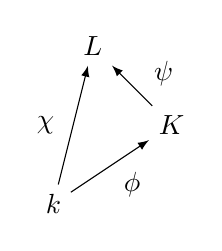
\begin{tikzpicture}
  \node (E) at (0, 0) {$k$};
  \node (F) at (1.5, 1) {$K$};
  \node (G) at (0.5, 2) {$L$};

  \draw[arrow] (E) -- (F);
  \draw[arrow] (E) -- (G);
  \draw[arrow] (F) -- (G);

  \node (f12) at (1, 0.25)
  {$\phi$};
  \node (f13) at (-0.1, 1)
  {$\chi$};
  \node (f23) at (1.4, 1.65)
  {$\psi$};
\end{tikzpicture}
\end{center}
The general problem, as well as additional sub-goals, are presented in
Section~\ref{sec:compatibility-problem}.

In Section~\ref{sec:conway}, we present a first solution, based on the Conway
polynomials~\cite{Parker90, Scheerhorn92}. These polynomials are used to define
the finite field extensions and possess the very interesting property of being
\emph{norm-compatible}, meaning that taking the norm of the root of a Conway
polynomial sends it to the root of another Conway polynomial. This provides
easy-to-compute embeddings: indeed the embedding description problem is solved
by computing a norm. Naturally, before using Conway polynomials, we first need
to compute them. This is a problem because we do not know any efficient
algorithm to compute Conway polynomials. As a consequence, Conway polynomials
are usually precomputed up to some degree $d$ in most computer algebra systems,
and it is no longer possible to compute embeddings with finite field extensions
that have a degree larger than this given degree $d$.

In Section~\ref{sec:bosma-canon-steel}, we introduce another solution to the
compatibility problem, called the Bosma-Canon-Steel framework~\cite{BCS97}.
This framework allows us to use any given polynomial to define our finite field
extensions, and is \emph{incremental}, meaning that we can always add more
extensions to our data structure, without having to recompute anything. It is
much more flexible than Conway polynomials, and is thus a very interesting
alternative to them. We describe it in details in Section~\ref{sec:bcs-alg}.
This framework was first available in the computer algebra system
Magma~\cite{Magma} since at least 1997. To the best of my knowledge, the only
additional computer algebra system using the Bosma-Canon-Steel framework is
Nemo~\cite{Nemo}. The framework was implemented in Fall 2019 and all the
implementation details, as well as experimental results, are given in
Section~\ref{sec:bcs-implem}.

\paragraph{Standard lattice of compatibly embedded finite field.}
Finally, in Chapter~\ref{chap:standard}, we construct a new method~\cite{DRR19}
for computing lattices of compatibly embedded finite fields, that is halfway
between the Conway polynomials and the Bosma-Canon-Steel framework. The central
element of this construction is the Lenstra-Allombert embedding algorithm. In
Section~\ref{sec:lenstra-allombert-embeddings}, we explain how this algorithm
can be used to produce compatible embeddings, by choosing compatible solutions
of~\eqref{eq:h90-kummer}, and the new challenges it raises.

In Section~\ref{sec:standard-solution}, we show that some large Kummer algebras
called \emph{complete Kummer algebras}, that can be described by
\[
  A_{p^a-1} = \mathbb{F}_{p^{p^a-1}}\otimes\mathbb{F}_{p}(\zeta_{p^a-1})
  = \mathbb{F}_{p^{p^a-1}}\otimes \mathbb{F}_{p^a},
\]
admit special solutions of~\eqref{eq:h90-kummer}, that we call \emph{standard
solutions}. We then prove that from these standard solutions in the complete
algebra $A_{p^a-1}$, we can deduce solutions of~\eqref{eq:h90-kummer} in every
Kummer algebra
\[
  A_n = \mathbb{F}_{p^n}\otimes \mathbb{F}_{p}(\zeta_n)
\]
such that $\mathbb{F}_{p}(\zeta_n)$ is an extension of degree $a$. We see that
the solutions derived from the standard solution also share some special
properties, and that all these solutions can be used to obtain
compatible embeddings between all the associated finite field extension
$\mathbb{F}_{p^n}$.

In Section~\ref{sec:towards-standard-embeddings}, we show that if $a\mid b$, the solutions
of~\eqref{eq:h90-kummer} in the complete Kummer algebras $A_{p^a-1}$ and
$A_{p^b-1}$ can also be linked by some operator that we call \emph{scalar norm
operator} and that essentially acts like the usual norm of finite fields.
We use these results in Section~\ref{sec:standard-embeddings} to obtain
compatible embeddings between arbitrary finite field extensions
$\mathbb{F}_{p^m}$ and $\mathbb{F}_{p^n}$, provided that $m\mid n$.

We analyze the complexity of this new framework in
Section~\ref{sec:implementation-std-lattices} and provide an implementation in
the Julia programming language~\cite{Julia}, using Nemo. We see that our
construction is practical, and that embeddings are computed in a reasonable
time. In Section~\ref{sec:perspectives}, we discuss the limitations of our
approach and propose new perspectives of research.


\part{Efficient arithmetic in a single finite field}
\label{part:single}

\chapter{Preliminary}
\label{chap:preliminary}
Throughout all this document, we will use a lot of results from algebra. This
chapter is here to sum up these results and try to maintain the illusion that
this thesis is self-contained. The reader familiar with the notions of finite
fields, algebraric function fields, complexity model may very well skip this
chapter.

\section{Finite fields}
Finite fields are ubiquitous in cryptography and coding theory, probably because
their field structure, a rigid one, allows to understand how they work, and
their finiteness makes them easier to represent on a computer. They are also
everywhere in this thesis, and are probably on almost every paper I
wrote on during these last three years. They are quite important.

\section{Algebraic function fields}
\section{Complexity model}
We use \cite{GG13}.


\chapter{Bilinear complexity and Chudnosky$^2$-type algorithms}
\label{chap:bilinear}
\section{Evaluation - Interpolation}
\section{Complexities}


\chapter{Hypersymmetric bilinear complexity}
\label{chap:hypersymmetric}
In Chapter~\ref{chap:bilinear}, we have seen the notions of bilinear complexity
and symmetric bilinear complexity. We now investigate even stronger
notions of symmetry, allowing to have very short representations of a bilinear
map.

\minitoc

% TODO
% ====
%
% Find a nice picture to put here to illustrate something in link with the
% chapter.

\clearpage
\section{Symmetric and hypersymmetric fomulas}
% Table of content
% ================
%
% - Recall of the definition of symmetric
% - Existence and lemma for the symmetric case
% - non degenerate bilinear form, link with the trace, but not only
% - Link between symmetric and hypersymmetric in smaller dimension
% - Galois invariance
% - Comment for the case of the particular algebras we study, what is known and
%   what is not
%
% Comment
% =======
%
% Comment about the trisymmetric formulas, it is true that F_4/F_2 can be
% represented by a trisymmetric formula but it is not the case for F_8/F_2. We
% should check the lemma saying something on the existence of the trisymmetric
% decomposition, but it is probably just simpler.

Let $\K$ be a finite field, $V_1$, $V_2$ and $W$ three finite-dimensional $\K$-vector
space and
\[
  \Phi:V_1\times V_2\to W
\]
a bilinear map. Recall Definition~\ref{defi:bilinear-formula}:
\[
  \Phi(x, y) = \sum_{j=1}^t\varphi_j(x)\psi_j(y)w_j,
\]
where for all $1\leq j\leq t$, $\varphi_j\in V_1^\vee$ and $\phi_j\in V_2^\vee$ are linear forms and
$w_j\in W$ is a vector, is called a \emph{bilinear formula} of length $t$. If
the spaces $V_1$ and $V_2$ are equal and if the bilinear map $\Phi$ is
symmetric, \ie if for all $x, y\in V$
\[
  \Phi(x, y) = \Phi(y, x),
\]
we can investigate the existence of formulas satisfying the same condition of
symmetry, \ie formulas where for all $1\leq j\leq t$, $\varphi_j=\psi_j$,
resulting in \emph{symmetric} bilinear form:
\[
  \Phi(x, y) = \sum_{j=1}^t\varphi_j(x)\varphi_j(y)w_j.
\]
In fact, we can define other interesting types of symmetries, but it is useful
to first generalize the notions that we saw in Chapter~\ref{chap:bilinear} to
higher dimensions.
\subsection{Generalization to multilinear maps}
The definitions of bilinear formula and bilinear complexity are not bound to the
bilinear case and can be generalized to arbitrary dimension. These general
definitions will be used in Section~\ref{subsec:trisym} to define
\emph{hypersymmetric} complexity.
\begin{defi}[Multilinear formula]
Let $V_1, V_2, \dots, V_s$ and $W$ be $s+1$ finite-dimensional $\K$-vector
spaces and
\[
  \Phi:V_1\times V_2\times\dots\times V_s\to W
\]
an $s$-linear map. A \emph{multilinear formula}, or \emph{multilinear
decomposition}, or \emph{multilinear algorithm} of length $t$ for $\Phi$ is a
collection of $s\times t$ linear forms $\varphi_1^{(1)}, \varphi_2^{(1)}, \dots,
\varphi_t^{(1)}\in V_1^\vee$ up to $\varphi_1^{(s)}, \varphi_2^{(s)}, \dots,
\varphi_t^{(s)}\in V_s^{\vee}$ and $t$ vectors $w_1, \dots, w_t$, such that for all $x_1\in V_1, \dots, x_s\in
V_s$, we have
\[
  \Phi(x_1, \dots, x_s) =
  \sum_{j=1}^t\varphi_j^{(1)}(x_1)\dots\varphi_j^{(s)}(x_s)w_j.
\]
\end{defi}
\begin{defi}[Multilinear complexity]
Let $V_1, V_2, \dots, V_s$ and $W$ be $s+1$ finite-dimensional $\K$-vector
spaces and
\[
  \Phi:V_1\times V_2\times\dots\times V_s\to W
\]
an $s$-linear map. The \emph{multilinear complexity} $\mu(\Phi)$ of $\Phi$ is the
minimal length $t$ of a multilinear formula for $\Phi$.
\end{defi}
As in the case of bilinear complexity, the multilinear complexity $\mu(\Phi)$ of a
multilinear map $\Phi$ can also be defined as the rank of the tensor in 
\[
  V_1^\vee\otimes\dots\otimes V_s^\vee\otimes W
\]
corresponding to $\Phi$, see Example~\ref{ex:bilinear-complexity} for an
illustration of this correspondence in the bilinear case. In the case where
\[
  V_1 = V_2 = \dots = V_s,
\]
symmetric formulas and
symmetric complexity can also be generalized when $\Phi$ is a \emph{symmetric}
multilinear map, \ie when for all permutation $\sigma\in\mathfrak S_s$ and for
all vectors $x_1, \dots, x_s\in V$, we have
\[
  \Phi(x_1, \dots, x_s) = \Phi(\sigma(x_1), \dots, \sigma(x_s)).
\]
\begin{defi}[Symmetric multilinear formula]
Let $V$ and $W$ be two finite-dimensional $\K$-vector
spaces and
\[
  \Phi:\underset{\textrm{$s$ times}}{\underbrace{V\times\dots\times V}}\to W
\]
a symmetric $s$-linear map. A \emph{symmetric multilinear formula}, or
\emph{symmetric multilinear
decomposition}, or \emph{symmetric multilinear algorithm} of length $t$ for $\Phi$ is a
collection of $t$ linear forms $\varphi_1, \varphi_2, \dots,
\varphi_t\in V^\vee$ and $t$ vectors $w_1, \dots, w_t$, such that for all $x_1, \dots, x_s\in
V$, we have
\[
  \Phi(x_1, \dots, x_s) =
  \sum_{j=1}^t\varphi_j(x_1)\dots\varphi_j(x_s)w_j.
\]
\end{defi}
\begin{defi}[Symmetric multilinear complexity]
Let $V$ and $W$ be two finite-dimensional $\K$-vector
spaces and
\[
  \Phi:\underset{\textrm{$s$ times}}{\underbrace{V\times\dots\times V}}\to W
\]
a symmetric $s$-linear map. The \emph{symmetric multilinear complexity} $\musym(\Phi)$ of $\Phi$ is the
minimal length $t$ of a symmetric multilinear formula for $\Phi$. If no such
formula exists, we set
\[
  \musym(\Phi) = \infty.
\]
\end{defi}
Contrary to the bilinear case, some symmetric multilinear maps do not admit a symmetric
decomposition, but the problem of whether a symmetric multilinear map admits
a symmetric multilinear formula is well understood and follows from
Theorem~\ref{thm:symmetric-formula}.
\begin{thm}[{\cite[Thm.~A.7]{Randriam15}}]\label{th:criterion}
\label{thm:symmetric-formula}
Let $\Phi:V^s\to W$ be a $s$-linear map between finite dimensional vector spaces over $\mathbb{F}_q$.
Then $\Phi$ admits a symmetric decomposition if and only if $\Phi$ is \emph{Frobenius-symmetric},
\ie if and only if it is symmetric and one of the following two conditions holds:
\begin{itemize}
\item $s\leq q$
\item $s\geq q+1$ and for all $u,v,z_1,\dots,z_{s-q-1}$ in $V$,
\[
\Phi(\underset{\textrm{$q$ times}}{\underbrace{u,\dots,u}},v,z_1,\dots,z_{s-q-1})=\Phi(u,\underset{\textrm{$q$ times}}{\underbrace{v,\dots,v}},z_1,\dots,z_{s-q-1}).
\]
\end{itemize}
\end{thm}

\subsection{Trisymmetric and hypersymmetric complexity}
\label{subsec:trisym}

Under even stricter conditions, we can study the existence of even more
symmetric formulas. These formulas allow to describe a multilinear map with
fewer elements, and thus give a compact definition of the map. Since the
symmetry conditions are stronger there are fewer such formulas, and as a
consequence the search space is smaller. Thus, we expect algorithms to be
faster, as was the case when using Barbulescu \etal algorithm
(Algorithm~\ref{algo:BDEZ}) to find symmetric formulas. Let us define those
``stricter conditions''. Let
\[
  \Phi:V^s\to V
\]
be an $s$-linear symmetric map, \ie we additionnaly ask that $W=V$. We also
assume that $V$ has a non-degenerate symmetric bilinear form, that we write as a
scalar product
\[
 \begin{array}{ccc}
 V\times V &\to&\K\\
 (v,w)&\mapsto&\ps{v}{w}.
 \end{array}
\]
In that case, we know that the vector space $V$ is isomorphic to its dual space
$V^\vee$:
\[
  V\cong V^\vee,
\]
\ie for each linear form $\varphi\in V^\vee$, there exist a unique vector $a\in
V$ such that for all $x\in V$, we have
\[
  \varphi(x) = \ps{a}{x}.
\]
Under these conditions, we can now write a symmetric formula for $\Phi$ as
\[
  \Phi(x, y) = \sum_{j=1}^t\ps{a_i}{x}\ps{a_i}{y}w_j
\]
where for all $1\leq j\leq t$, $a_j\in V$ is a vector of $V$. As a consequence,
we can also describe a symmetric formula for $\Phi$ as the data of vectors
$(a_j)_{1\leq j\leq t}$ and $(w_j)_{1\leq j\leq t}$. In order to have an even
more compact description of $\Phi$, one can ask for the vectors $w_j$ to be
proportional to $a_i$, leading to the definition of hypersymmetric
formula.
% Note
% ====
%
% But is that really natural? Wouldn't it be better to say that we would like
% the a_i and the b_i to be equal? 
%
% TODO
% ====
%
% Maybe change this to include the case a_i = b_i and discuss it a little, or
% maybe not, we'll see.

\begin{defi}[Hypersymmetric formula]
Let $V$ a finite-dimensional $\K$-vector
spaces equipped with a saclar product and
\[
  \Phi:\underset{\textrm{$s$ times}}{\underbrace{V\times\dots\times V}}\to W
\]
a symmetric $s$-linear map. A \emph{hypersymmetric formula}, or
\emph{hypersymmetric decomposition}, or \emph{hypersymmetric algorithm} of length $t$ for $\Phi$ is a
collection of $t$ vectors $a_1, \dots, a_t\in V$ and $t$ scalars $\lambda_1,
\dots, \lambda_t\in\K$, such that for all $x_1, \dots, x_s\in
V$, we have
\[
  \Phi(x_1, \dots, x_s) =
  \sum_{j=1}^t\lambda_j\ps{a_j}{x_1}\dots\ps{a_j}{x_s}a_j.
\]
\end{defi}
\begin{defi}[Hypersymmetric complexity]
Let $V$ be a finite-dimensional $\K$-vector spaces equipped with a saclar product
and
\[
  \Phi:\underset{\textrm{$s$ times}}{\underbrace{V\times\dots\times V}}\to W
\]
a symmetric $s$-linear map. The \emph{hypersymmetric complexity} $\muhyp(\Phi)$ of $\Phi$ is the
minimal length $t$ of a hypersymmetric formula for $\Phi$. If no such
formula exists, we set
\[
  \muhyp(\Phi) = \infty.
\]
\end{defi}
\begin{ex}
  We take the same case as in Example~\ref{ex:bilinear-complexity}, but viewed
  a bit differently. Let $\K=\mathbb{F}_2$ and 
  \[
    V=\mathbb{F}_4\cong\mathbb{F}_2[T]/(T^2+T+1)\cong\mathbb{F}_2(\zeta)
  \]
  seen as a $\mathbb{F}_2$-vector space of dimension $2$ using the base $(1,
  \zeta)$. The $\mathbb{F}_2$-bilinear map $\Phi$ that we
  consider is the product in $\mathbb{F}_4$:
  \[
 \begin{array}{cccc}
   \Phi: & \mathbb{F}_4\times \mathbb{F}_4 &\to&\mathbb{F}_4\\
 &(x,y)&\mapsto&xy.
 \end{array}
  \]
  We also consider the non-degenerate symmetric bilinear form
\[
 \begin{array}{ccc}
   \mathbb{F}_4\times \mathbb{F}_4 &\to&\mathbb{F}_2\\
 (v,w)&\mapsto&\tr(vw),
 \end{array}
\]
where $\tr$ is the trace of the field extension $\mathbb{F}_4/\mathbb{F}_2$,
and we write
\[
  \tr(xy) = \ps{x}{y}.
\]
If $x = x_0 + x_1\zeta\in\mathbb{F}_4$ is an element in the extension field, we have $\tr(x) = x_1$, and if $y = y_0
+ y_1\zeta\in\mathbb{F}_4$ is another element, then their product is
\[
  xy = x_0y_0 + x_1y_1 + (x_0y_1 + x_1y_0 + x_1y_1)\zeta.
\]
We also see that
\[
\left\{ 
  \begin{array}{lll}
    \ps{1}{x}\ps{1}{y} &=& x_1y_1 \\
    \ps{1+\zeta}{x}\ps{1+\zeta}{y} &=& x_0y_0 \\
    \ps{\zeta}{x}\ps{\zeta}{y} &=& (x_0+x_1)(y_0+y_1)
  \end{array}
\right.
\]
and thus we have
\[
  xy =
  \ps{1}{x}\ps{1}{y}\cdot1+\ps{1+\zeta}{x}\ps{1+\zeta}{y}\cdot(1+\zeta)+\ps{\zeta}{x}\ps{\zeta}{y}\cdot\zeta.
\]
This is an hypersymmetric formula of length $3$, and we can prove that there are
no formulas of length $2$, so we have
\[
  \muhyp(\Phi) = 3.
\]
This is in fact the very same formula as in
Example~\ref{ex:bilinear-complexity}.
\end{ex}
In order to investigate the existence of hypersymmetric decompositions, we
remark that there is a natural link between hypersymmetric decompositions of 
the $s$-linear map
\[
  \Phi:V^s\to V
\]
and symmetric decompositions of the $(s+1)$-linear form $\widetilde\Phi$ defined by
\[
  \begin{array}{llll}
    \widetilde\Phi:&V^{s+1}&\to&\K\\
    &(x_1, \dots, x_{s+1})&\mapsto&\ps{\Phi(x_1, \dots, x_s)}{x_{s+1}}
  \end{array}
\]
in the sense of~Lemma~\ref{lm:link-hyp-sym}. Moreover, we say that the
$s$-linear map $\Phi$ is \emph{hypersymmetric} if the associated $(s+1)$-linear
form $\widetilde\Phi$ is symmetric.
\begin{lm}
  \label{lm:link-hyp-sym}
  Let $V$ a $\K$-vector space and 
  \[
    \Phi:V^s\to V
  \]
  a symmetric $s$-linear map. 
Elements $(a_j)_{1\leq j\leq t}$ in $V$ and scalars $(\lambda_j)_{1\leq j\leq t}$ in $\K$ define a hypersymmetric formula for the $s$-linear map $\Phi$,
\[
\Phi(x_1,\dots,x_s)=\sum_{j=1}^{t}\lambda_j\ps{a_j}{x_1}\cdots\ps{a_j}{x_t}a_j,
\]
if and only if they define a symmetric formula for the $(s+1)$-linear form $\widetilde{\Phi}$,
\[
\widetilde{\Phi}(x_1,\dots,x_s,x_{s+1})=\sum_{j=1}^{t}\lambda_i\ps{a_j}{x_1}\cdots\ps{a_j}{x_t}\ps{a_j}{x_{s+1}}.
\]

Thus, $\Phi$ admits a hypersymmetric formula if and only if $\widetilde{\Phi}$ is Frobenius-symmetric (in the sense of Theorem~\ref{thm:symmetric-formula}),
and we have
\[
\muhyp(\Phi)=\musym\left(\widetilde{\Phi}\right).
\]

In particular, if $q\geq s+1$, then any hypersymmetric $s$-linear map over $\mathbb{F}_q$ admits a hypersymmetric formula.
\end{lm}
\begin{proof}
  Assume that $\Phi$ admits a hypersymmetric decomposition, such that for all
  $x_1, \dots, x_s\in V$, we have
  \[
    \Phi(x_1,\dots,x_s)=\sum_{j=1}^{t}\lambda_i\ps{a_j}{x_1}\cdots\ps{a_j}{x_t}a_j,
  \]
  then, by taking the scalar product with any $x_{s+1}$, we obtain
\[
  \ps{\Phi(x_1, \dots,
  x_s)}{x_{s+1}}=\widetilde{\Phi}(x_1,\dots,x_s,x_{s+1})=\sum_{j=1}^{t}\lambda_i\ps{a_j}{x_1}\cdots\ps{a_j}{x_t}\ps{a_j}{x_{s+1}},
\]
which defines a symmetric decomposition for $\widetilde\Phi$. In the other
direction, assume that $\widetilde\Phi$ admits a symmetric decomposition, such
that for all $x_1, \dots, x_{s+1}\in V$, we have
\[
\widetilde{\Phi}(x_1,\dots,x_s,x_{s+1})=\sum_{j=1}^{t}\lambda_i\ps{a_j}{x_1}\cdots\ps{a_j}{x_t}\ps{a_j}{x_{s+1}}.
\]
It can also be written as
\[
  \ps{\Phi(x_1, \dots,
  x_s)}{x_{s+1}}=\ps{\sum_{j=1}^t\lambda_j\ps{a_j}{x_1}\cdots\ps{a_j}{x_s}a_j}{x_{s+1}},
\]
so that we have
\[
  \ps{\Phi(x_1, \dots,
  x_s)-\sum_{j=1}^t\lambda_j\ps{a_j}{x_1}\cdots\ps{a_j}{x_s}}{x_{s+1}}=0.
\]
Since the scalar product $\ps{\cdot}{\cdot}$ is non-degenerate, it means that
  \[
    \Phi(x_1,\dots,x_s)=\sum_{j=1}^{t}\lambda_i\ps{a_j}{x_1}\cdots\ps{a_j}{x_t}a_j.
  \]
  Hence $\Phi$ admits a hypersymmetric decomposition. The other assertions
  follow.
\end{proof}
The most important case is arguably the bilinear case, where $s=2$, because it
was thoroughly studied. For that reason, we sometimes replace the word
hypersymmetric by \emph{trisymmetric} in that particular case, because of the
form of the formulas
\[
  \Phi(x, y) = \sum_{j=1}^t\lambda_j\ps{a_j}{x}\ps{a_j}{y}a_j
\]
that includes the same element $a_j$ three times, and we write $\mutri(\Phi)$
instead of $\muhyp(\Phi)$. Lemma~\ref{lm:link-hyp-sym} states that, if $q\geq3$, a
trisymmetric map $\Phi$ always admits a trisymmetric decomposition.

\subsection{Galois invariance}

\section{Algorithmic seach in small dimension}
\section{Asymptotic complexities}


\part{Efficient arithmetic in a lattice of finite fields}
\label{part:lattice}

\chapter{Isomorphism algorithms}
\label{chap:isomorphism}
We studied in Part~\ref{part:single} the arithmetic of a single finite field
extension. We now study a set of several extensions. The very first step will be
to understand how to compute an isomorphism (or an embedding) between two finite
fields: that is the material of this chapter.
\minitoc

% TODO: figure

\clearpage

Our reference for this chapter is~\cite{BDDFS17}: we cover a subpart of the
paper because we are interested in the naive isomorphism algorithm (used in
Chapter~\ref{chap:lattice}) and Allombert's algorithm (used in
Chapter~\ref{chap:standard}). We thus do not cover all the isomorphism
algorithms, the reader interested in Rains' algorithm and its elliptic variant
can take a look at the paper cited above.

\section{Generalities and naive algorithm}

Even if our real goal is to compute \emph{embeddings} of finite fields, \ie
ring homomorphisms
\[
  \phi:K\to L
\]
with $K$ and $L$ finite fields, we often refer to the algorithms as
\emph{isomorphism} algorithms. Indeed, computing the embedding $\phi$ is
the same as computing an isomorphism
\[
  \phi':K\to K'
\]
where $K\cong K'$ is isomorphic to a subfield $K'\subset L$ of $L$. The
isomorphism $\phi'$ is just the embedding $\phi$ with its codomain being
restricted to $K'$.

\subsection{Description of the problem}

We let $p$ be a prime number, $\K = \mathbb{F}_p$ be the field with $p$ elements,
and $f, g\in\K[X]$ two irreducible polynomials with
\[
  m=\deg f\mid\deg g=n.
\]
Let
\[
  K=\K[X]/(f(X))\cong\mathbb{F}_{p^m}
\]
and
\[
  L = \K[Y]/(g(Y))\cong\mathbb{F}_{p^n}
\]
two extensions of $\K$. We know there is an embedding
\[
  \phi:K\to L,
\]
unique up to $\K$-automorphism of $K$, \ie there are
\[
  \Card\Gal(K/\K)=m
\]
different embeddings from $K$ to $L$, than can be described as
\[
  \phi\circ\sigma
\]
for $\sigma\in\Gal(K/\K)$. Equivalently, they can also be described as
\[
  \sigma'\circ\phi
\]
with $\sigma'\in\Gal(\phi(K)/\K)$. The \emph{embedding problem} is then to
efficiently find, represent and evaluate one such embedding $\phi$. The problem
is split in two sub-parts.
\begin{description}
  \item[Embedding description problem.] Compute elements $\alpha\in K$ and
    $\beta\in L$ such that 
    \[
      K=\K(\alpha)
    \]
    and such that there exists an embedding $\phi$ mapping $\alpha$ to $\beta$.
  \item[Embedding evaluation problem.] Given elements $\alpha$ and $\beta$
    defined above, and elements $\gamma\in K$, $\delta\in L$, solve the
    following problems:
    \begin{itemize}
      \item compute $\phi(\gamma)\in L$;
      \item test if $\delta\in\phi(K)$;
      \item if $\delta\in\phi(K)$, then compute $\phi^{-1}(\delta)\in K$.
    \end{itemize}
\end{description}
As the name suggests, the \emph{embedding description problem} focuses on
finding a pair of elements that are sufficient to describe an embedding. Indeed,
if 
\[
  K=\K(\alpha)
\]
we know that every element $x\in K$ can be uniquely written as 
\[
  x = \sum_{j=0}^{m-1}a_j\alpha^j
\]
with $a_j\in\K$ for al $0\leq j\leq m-1$, and the embedding $\phi$ is then
defined by
\[
  \phi(x) = \sum_{j=0}^{m-1}a_j\beta^j.
\]
\begin{prop}
  \label{prop:description}
 The elements $\alpha$ and $\beta$
 describe an embedding if and only if they have the same minimal polynomial. 
\end{prop}
\begin{proof}
  Let $\phi:K\to L$ be an embedding mapping $\alpha$ to $\beta$ and let 
  \[
    P = \Minpoly_\K(\alpha)
  \]
  be the the minimal polynomial of $\alpha$. Then 
  \begin{align*}
    P(\beta) &= P(\phi(\alpha)) \\
    &= \phi(P(\alpha))\\
    &= \phi(0) \\
    &= 0
  \end{align*}
  thus $\Minpoly_\K(\beta)\neq 1$ divides $P$ which is irreducible so 
  \[
\Minpoly_\K(\beta) = P.
  \]
 Conversely, if $\alpha$ and $\beta$ have the same minimal polynomial $P$, then the
 map $\phi$ is well-defined and defines an isomorphism between the fields $\K(\alpha)$ and
 $\K(\beta)$, that are both isomorphic to the field
 \[
   \K[X]/(P(X)).
 \]
\end{proof}
While the first problem focuses on finding a description of $\phi$, the
\emph{embedding evaluation problem} independently asks how to efficiently use
the description to compute the actual embedding. We target this question in
Section~\ref{sec:evaluation}.

\subsection{Embedding description problem and naive algorithm}

Until the end of this section and in Section~\ref{sec:allombert}, we deal with
the \emph{embedding description problem}, although we only review a subpart of
the existing algorithms (see~\cite{BDDFS17} for other algorithms). As above, let
$f$ and $g$ two irreducible polynomials with coefficients in $\K$ such that
\[
  m=\deg f\mid \deg g=n.
\]
and let
\[
  K=\K[X]/(f(X))\cong\mathbb{F}_{p^m}
\]
and
\[
  L = \K[Y]/(g(Y))\cong\mathbb{F}_{p^n}
\]
two finite fields. Then one can simply take $\alpha$ to be the class of $X$ in
$K$ and choose $\beta$ to be any root of $f$ in $L$. Indeed, we know that there
is an isomorphic copy of $K$ in $L$ and thus that $f$ splits over $L$.
Furthermore, any root of $f$ will have $f$ as its minimal polynomial, which is
also the minimal polynomial of $\alpha$ by construction. By
Proposition~\ref{prop:description}, the map 
\[
  \phi:K\to L
\]
sending $\alpha$ to $\beta$ is an embedding. The critical routine in that
algorithm is to find a root of $f$ in $L$, that can be done using Shoup-Kaltofen
\emph{equal degree factorization} algorithm~\cite{KS97}. The complexity analysis
of~\cite{BDDFS17} indicates that the cost is strictly larger than quasi-quadratic
complexity $\tilde O(m^2)$. A more efficient algorithm, due to Lenstra and
Allombert, is discussed in Section~\ref{sec:allombert}.

\section{Lenstra-Allombert algorithm}
\label{sec:allombert}

Both Lenstra~\cite{Lenstra91} and Allombert used
Kummer theory, the study of certain field extensions, to compute isomorphisms
between finite fields. But while Lenstra's focus
was on proving the existence of a deterministic isomorphism algorithm, Allombert 
wanted to provide a practical algorithm. This led to the invention of the
Lenstra-Allombert algorithm~\cite{Allombert02} in 2002, for which we give a
description in this section. The ideas of Allombert play an important part in
Chapter~\ref{chap:standard} too. The techniques based on Kummer theories work
for extensions of degree $n$ coprime to the characteristic $p$. In order to have
an algorithm working for any type of extension, the solution is to deal with the
part of the extension which degree is divisible by $p$ separately using
Artin-Shreier theory and to glue the results together in the end.

% TODO
% ====
%
% Add a part on Artin-Shreier?


\subsection{Preliminaries}
\label{sec:preliminaries}

Let us first discuss a simpler case than the general one, that will highlight
the method behind Lenstra-Allombert isomorphism algorithm. Let $K$ and $L$ be
two finite fields of cardinality $p^n$, such that
\[
  K\cong L\cong \mathbb{F}_{p^n}.
\]
Assume that $\gcd(p, n)=1$ and that
\[
  n\mid p-1,
\]
or equivalently that there is a primitive $n$-th root of unity in
$\K=\mathbb{F}_p$, that we denote by $\zeta$. The algorithm is based on
Proposition~\ref{prop:h90}.

\begin{prop}[Hilbert $90$ theorem]
  \label{prop:h90}
  Let $K$ be a finite extension of $\K=\mathbb{F}_p$ of degree $n$ such that there exists a
primitive $n$-th root of unity $\zeta\in\K$ in the base field $\K$, \ie such
that $n$ divides $p-1$. 
 Let $\sigma$ be the generator of the Galois group of the extension
 \[
   K/\K
 \]
 and consider the following equation in $K$.
 \begin{equation}
   \tag{H90}
   \sigma(x) = \zeta x
   \label{eq:h90}
 \end{equation}
The solutions of~\eqref{eq:h90} form a one dimensional $\K$-vector space and if
$\alpha\in K$ is such a solution, we have
\[
  \alpha^n\in\K.
\]
If $\alpha$ is also nonzero, then it is a generator of $K$ over $\K$.
\end{prop}
\begin{proof}
  Let us first construct a nonzero solution of~\eqref{eq:h90}. Consider the polynomial
  \[
    P = \sum_{j=0}^{n-1}\zeta^{-j} X^{p^j}
  \]
  of degree $p^{n-1}$. The polynomial $P$ has at most $p^{n-1}$ roots in $K$,
  which has cardinality $p^n$, so there exists some element $x\in K$ such that
  \[
    y = P(x)\neq0.
  \]
  Now, by construction, we have
  \begin{align*}
    \sigma(y) &= \sigma(\sum_{j=0}^{n-1}\zeta^{-j}x^{\sigma^{j}})\\
    &= \sum_{j=0}^{n-1}\zeta^{-j}x^{\sigma^{j+1}}\\
    &= \zeta \times \sum_{j=0}^{n-1}\zeta^{-(j+1)}x^{\sigma^{j+1}}\\
    &= \zeta \times \sum_{j=1}^{n}\zeta^{-j}x^{\sigma^{j}}\\
    &= \zeta y
  \end{align*}
  and thus $y$ is a nonzero solution of~\eqref{eq:h90}. All the elements
  \[
    \lambda y
  \]
  with $\lambda\in\K$ are also solution of~\eqref{eq:h90} since
  \[
    \sigma(\lambda y) = \lambda\sigma(y) = \zeta\lambda y,
  \]
  and the equation has at most $p$ solutions because the polynomial
  \[
    X^p - \zeta X
  \]
  has at most $p$ roots in $K$. Thus there are exactly $p$ different solutions,
  that are the elements of $\Vect(y)$. Let $z$ be a solution of~\eqref{eq:h90},
  then we have
  \begin{align*}
   \sigma(z^n) &= \sigma(z)^n\\
   &= (\zeta z)^n\\
   &= z^n,
  \end{align*}
  therefore $z^n$ is fixed by $\sigma$, which means that
  \[
    z^n\in\K.
  \]
  If $z$ is also nonzero, then for all $0\leq j<n$, we have
  \begin{align*}
    \sigma^j(z) &= \underbrace{(\sigma\circ\dots\circ\sigma)}_{j\text{ times}}(z)\\
    &= \underbrace{(\sigma\circ\dots\circ\sigma)}_{j-1\text{ times}}(\zeta z)\\
    &= \zeta\underbrace{(\sigma\circ\dots\circ\sigma)}_{j-1\text{ times}}(z)\\
    &= \zeta^j z\\
    &\neq z.
  \end{align*}
  Consequently, $z$ is not in any subfield of $K$ and is thus a generator of $K$
  over $\K$.
\end{proof}
Note that Proposition~\ref{prop:h90} applies both to the fields $K$ and $L$,
therefore we can solve Equation~\eqref{eq:h90} in both fields. Let $\alpha_K$ be a
solution of Equation~\eqref{eq:h90} for the root $\zeta$ in $K$, and $\alpha_L$
a solution in $L$. Since we want the primitive $n$-th root of unity $\zeta$ to
be the same in $K$ and $L$, we assume that we already have an embedding from
$\K$ in both these fields. In practice, since $\K$ is a
prime field and the fields $K$ and $L$ are represented by polynomials over
$\K = \mathbb{F}_p=\mathbb{Z}/p\mathbb{Z}$, the assumption is not really
hard to meet. Let
\[
  a_K = \alpha_K^n
\]
and
\[
  a_L = \alpha_L^n.
\]
By Proposition~\ref{prop:h90}, we know that $a_K$ and $a_L$ are both in $\K$ and
this can be used to compute an isomorphism between $K$ and $L$.
\begin{prop}[Allombert~{\cite{Allombert02}}]
 The quotient
 \[
   a_K/a_L
 \]
 is an $n$-th power in $\K$, and if
 \[
   c^n = a_K/a_L
 \]
 then the map sending $\alpha_K$ to $c\alpha_L$ is an isomorphism from $K$ to $L$.
\end{prop}
\begin{proof}
  Let $\phi:K\to L$ be a $\K$-isomorphism between $K$ and $L$. We have
  \begin{align*}
    \sigma(\phi(\alpha_K)) &= \phi(\alpha_K)^p\\
    &= \phi(\alpha_K^p)\\
    &= \phi(\sigma(\alpha_K))\\
    &= \phi(\zeta\alpha_K)\\
    &= \zeta\phi(\alpha_K)
  \end{align*}
  thus $\phi(\alpha_K)$ is a solution of~\eqref{eq:h90} and by
  Proposition~\ref{prop:h90} there exists $\lambda\in\K$ such that
  \[
    \phi(\alpha_K) = \lambda\alpha_L.
  \]
  We also have
  \[
    \phi(\alpha_K)^n = \phi(\alpha_K^n) = \phi(a_K) = a_K,
  \]
  therefore the quotient
  \begin{align*}
    a_K/a_L &= \phi(\alpha_K)^n/\alpha_L^n\\
    &= \lambda^{n}
  \end{align*}
  is an $n$-th power in $\K$. Now let $c\in\K$ be any $n$-th root of $a_K/a_L$,
  then
  \[
    c = \zeta^j\lambda
  \]
  for some $0\leq j\leq n-1$, that is $c$ and $\lambda$ differ by a $n$-th root
  of unity, and so do $\phi(\alpha_K)$ and $c\alpha_L$:
  \[
    c\alpha_L = \zeta^j\phi(\alpha_K) = \sigma^j(\phi(\alpha_K)).
  \]
  Finally, the elements $c\alpha_L$ and $\phi(\alpha_K)$ have the same minimal
  polynomial, because they are conjugates, and $\phi(\alpha_K)$ has the same
  minimal polynomial as $\alpha_K$ because $\phi$ is an isomorphism, so by
  Proposition~\ref{prop:description}, the map sending $\alpha_K$ to $c\alpha_L$ is an
  isomorphism from $K$ to $L$.
\end{proof}
In this simpler case ($n$ divides $p-1$), Lenstra-Allombert algorithm consists
in
\begin{enumerate}
  \item finding $\alpha_K\in K$ and $\alpha_L\in L$ with
    $\sigma(\alpha_K)=\zeta\alpha_K$ and $\sigma(\alpha_L)=\zeta\alpha_L$;
  \item computing a $n$-th $c$ root of $\alpha_K^n/\alpha_L^n$;
  \item returning the embedding described by $\alpha_K\mapsto c\alpha_L$.
\end{enumerate}

\paragraph{General case.} When $n\nmid p-1$, which is always
the case asymptotically since $n>p-1$ at some point, there are no $n$-th roots
of unity in $\K$, and the strategy of Section~\ref{sec:preliminaries} cannot be
applied as if. Nevertheless, it is still possible to apply a similar idea by
extending the space so that it contains roots of unity.

\subsection{Kummer algebras}
\label{sec:kummer-algebras}

% TODO
% ====
%
% Fix the definitions by saying something about where do we pick the roots of
% unity from. Algebraic closure ? Doesn't that make some of the results trivial or
% something? 

Instead of ``just'' working in $\mathbb{F}_{p^n}$, we work in
\[
  A_n = \mathbb{F}_{p^n}\otimes \mathbb{F}_p(\zeta),
\]
where $\zeta$ is a primitive $n$-th root of unity, and where $\otimes$ is the tensor
product over $\K=\mathbb{F}_p$. We thus extend the scalars and force the existence of
suitable roots of unity. The $\K$-algebra $A_n$, that we call \emph{Kummer
algebra}, can now be used instead of
$\mathbb{F}_{p^n}$ in Lenstra-Allombert algorithm.

\begin{defi}[Kummer algebra]
 We call the $\K$-algebra
 \[
   A_n = \mathbb{F}_{p^n}\otimes\mathbb{F}_{p}(\zeta)
 \]
 a \emph{Kummer algebra of degree $n$}.
\end{defi}
\begin{defi}[Field of scalars]
  Let $A_n$ be a Kummer algebra of degree $n$. Then we define
  $\mathbb{F}_{p}(\zeta)$ as the \emph{field of scalars} of $A_n$, and we
  define the \emph{level} $\nu(n)$ of $A_n$ as
  \[
    \nu(n) = \mathrm{ord}_{(\mathbb{Z}/n\mathbb{Z})^\times}(p) = \left[
      \mathbb{F}_{p}(\zeta):\K \right],
  \]
  that is the degree of its field of scalars.
\end{defi}
Let $\sigma:x\mapsto x^p$ be the Frobenius automorphism of the extension
\[
  \mathbb{F}_{p^n}/\K,
\]
we extend it to $A_n$ by defining the linear map
\[
  \begin{array}{cccc}
    \sigma\otimes 1: & A_n & \to & A_n\\
    & \sum_j x_j\otimes y_j & \mapsto & \sum_j \sigma(x_j) \otimes y_j.
  \end{array}
\]
The map $\sigma\otimes 1$ will play the role of $\sigma$ in the simpler case.
\begin{lm}
  The map $\sigma\otimes1$ is a $1\otimes\mathbb{F}_{p}(\zeta)$-linear
  endomorphism with $n$ distinct eigenvalues, that are the powers of
  $1\otimes\zeta$.
\end{lm}
\begin{proof}
  Because of the linear independance of characters~\cite[Chapter VI,
  §4]{Lang04}, we know that the automorphisms
  \[
    \Id, \sigma, \sigma^2, \dots, \sigma^{n-1}
  \]
  are independant. We also know that 
  \[
    \sigma^n = \Id,
  \]
  therefore the minimal polynomial of the $\K$-linear endomorphism $\sigma$ is
  \[
    X^n-1.
  \]
  By the Cayley-Hamilton theorem, we deduce that the characteristic
  polynomial of $\sigma$ is also $X^n-1$. Now let $\B=\left\{ b_1, \dots, b_n \right\}$ be a basis of
  $\mathbb{F}_{p^n}/\K$ and let $M$ be the matrix of $\sigma$ in this basis.
  Then the matrix of the $1\otimes\mathbb{F}(\zeta)$-linear endomorphism
  $\sigma\otimes1$ in the basis
  \[
    \B\otimes 1 =\left\{ b_1\otimes1, \dots, b_n\otimes1 \right\}
  \]
  is also $M$. Thus, the characteristic polynomial of $\sigma\otimes1$ is again
  $X^n-1$, that splits completely in 
  \[
    1\otimes\mathbb{F}_{p}(\zeta)\cong \mathbb{F}_{p}(\zeta),
  \]
  the roots being the elements
  \[
    1\otimes\zeta^j
  \]
  for $0\leq j\leq n-1$. Finally, the eigenvalues are the roots of the
  characteristic polynomial so this concludes the proof.
\end{proof}
Since there are exactly $n$ distinct eigenvalues, we know that the
corresponding eigenspaces are all one-dimensional
$1\otimes\mathbb{F}_{p}(\zeta)$-vector spaces, and the eigenspace corresponding
to the eigenvalue $\zeta$ is described by the equation
 \begin{equation}
   \tag{H90}
   (\sigma\otimes1)(x) = (1\otimes\zeta) x
   \label{eq:h90-kummer}
 \end{equation}
 that we again denote by~\eqref{eq:h90-kummer}.
 \begin{lm}
   Let $\alpha$ be a nonzero solution of~\eqref{eq:h90-kummer} for the root
   $\zeta$. Then 
   \[
     \alpha^n\in 1\otimes\mathbb{F}_{p}(\zeta)
   \]
   and $\alpha$ is a generating element for $A_n$ as an algebra over
   $1\otimes\mathbb{F}_{p}(\zeta)$.
 \end{lm}


\section{The embedding evaluation problem}
\label{sec:evaluation}



\chapter{From a single finite field to plenty: lattice of embeddings}
\label{chap:lattice}
\section{Conway polynomials}
\section{Bosma-Canon-Steel framework}


\chapter{Standard lattices of compatibly embedded finite field}
\label{chap:standard}
We have seen in Chapter~\ref{chap:lattice} two independant methods to create
lattices of compatibly embedded finite fields. In this Chapter, we present a new
framework, inspired by both Conway polynomials and Bosma-Canon-Steel, that we
call \emph{standard lattice of compatibly embedded finite fields}.
\minitoc

% TODO: Figure

\clearpage
The two methods of Chapter~\ref{chap:lattice} both have their drawbacks: Conway
polynomials are expensive to compute and thus need to be precomputed, making
thme inefficient for large extensions, while Bosma-Canon-Steel needs more
computation each time an embedding is added in the lattice.
\section{Standard solution of Hilbert $90$}
\section{Standard embeddings}


\clearpage
\bibliographystyle{alpha}
\bibliography{erou}

\end{document}
